% PROSZĘ KOMPILOWAĆ TEN DOKUMENT ZA POMOCĄ SILNIKA XELATEX
% W PRZECIWNYM RAZIE NALEŻY USUNĄĆ PAKIET fontspec ORAZ USTAWIENIA FONTU
% Z PLIKU styles/prez_wmini_pl.sty (PIERWSZE TRZY LINIJKI)
% W PRZYPADKU BRAKU FONTU Adagio Slab NALEŻY ZGŁOSIĆ SIĘ DO BIP PW O JEGO UDOSTĘPNIENIE,
% ZAŁADOWAĆ INNY KRÓJ CZCIONKI LUB ZAKOMENTOWAĆ/USUNĄĆ USTAWIENIA FONTU

\documentclass[aspectratio=169]{beamer}

\usepackage{styles/prez_wmini_pl}
\usepackage{booktabs}
\setbeamertemplate{section in toc}[sections numbered]
\setbeamertemplate{subsection in toc}[subsections numbered]
\usepackage{times}
\usepackage{amsmath}
\usepackage{bm}

\usefonttheme[onlymath]{serif}

\definecolor{quotationcolour}{HTML}{F0F0F0}
\definecolor{quotationmarkcolour}{HTML}{1F3F81}

% Double-line for start and end of epigraph.
\newcommand{\epiline}{\hrule \vskip -.2em \hrule}
% Massively humongous opening quotation mark.
\newcommand{\hugequote}{%
  \fontsize{42}{48}\selectfont \color{quotationmarkcolour} \textbf{``}
  \vskip -.5em
}

% Beautify quotations.
\newcommand{\epigraph}[2]{%
  \bigskip
  \begin{center}
  \colorbox{quotationcolour}{%
    \parbox{.80\textwidth}{%
    \epiline \vskip 1em {\hugequote} \vskip -.5em
    \parindent 2.2em
    #1\vspace{-.25cm}\begin{flushright}\textsc{#2}\end{flushright}
    \epiline
    }
  }
  \end{center}
  \bigskip
}

\newcommand{\boldm}[1] {\mathversion{bold}#1\mathversion{normal}}

\graphicspath{ {./images/} }



% ------------------ Ustawienia użytkownika ------------------
% kolor tytułu prezentacji; zalecany white lub grafitowy.
% Poza tym można użyć zdefiniowanych w pakiecie kolorów:
% sloneczny, morelowy, mietowy, mokka, grafitowy, sliwkowy, szafirowy, wrzosowy
% lub wybrać sobie kolor z pakietu xcolor
\colorlet{title_color}{grafitowy}

\title{Opracowanie wirtualnego środowiska\\do symulacji dynamiki lotu\\ bezzałogowych statków powietrznych}
%\subtitle{Podtytuł consectetur adispiscing elit}
\author{Wojciech Gajda \and  Igor Faliszewski}
\date{9 stycznia 2024} % można tam wpisać datę jaką się chce lub zakomentować dla daty dzisiejszej



% ------------------ Początek prezentacji ------------------

\begin{document}
\sloppy

% Slajd tytułowy
{
\maketitleframe 
}

\begin{frame}
\frametitle{Agenda}
  \tableofcontents[  
    sectionstyle=show, 
    %hideallsubsections
    ]
\end{frame}

\begin{frame}
	\frametitle{Wymagania funkcjonalne}
	Role, aktorzy, funkcjonalności
\end{frame}

\begin{frame}
	\frametitle{Wymagania niefunkcjonalne}
\end{frame}

\begin{frame}
	\frametitle{Architektura I}
	\begin{itemize}
	\item UAV\_visualization
	\item UAV\_physic\_engine
	\item UAV\_controller
	\item UAV\_drop\_physic
	\item UAV\_common
	\item UAV\_server
	\item UAV\_map\_generator
	\end{itemize}
\end{frame}

\begin{frame}
	\frametitle{Architektura II}
	\begin{figure}
		\centering
		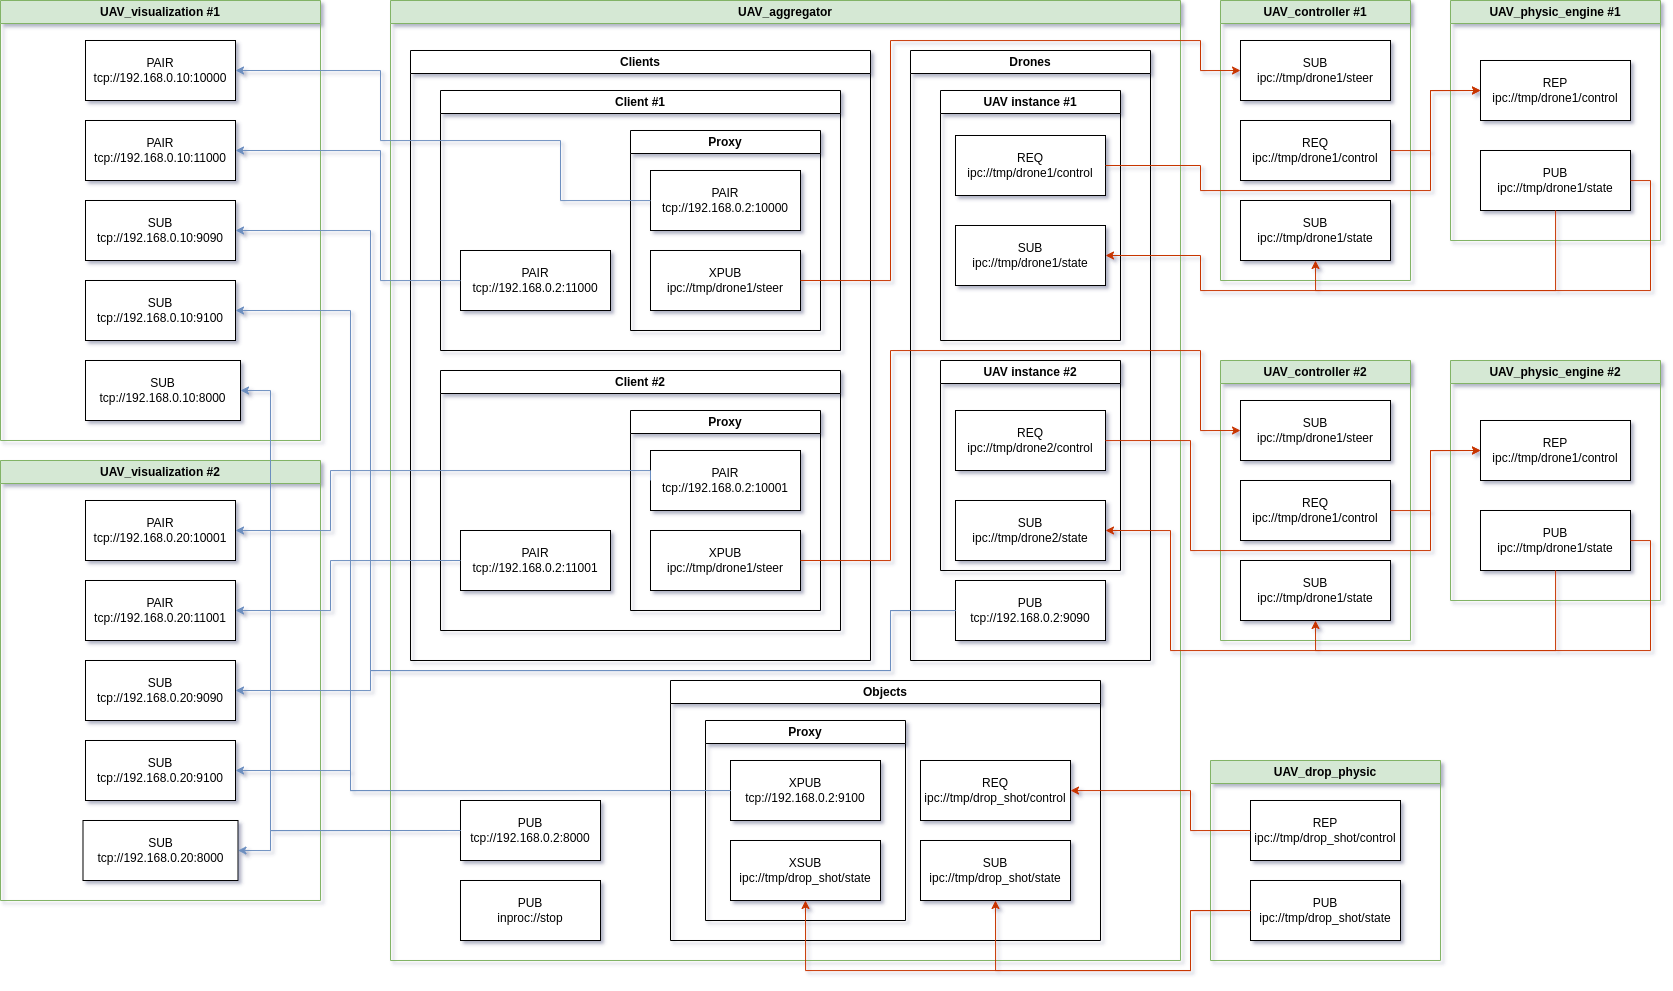
\includegraphics[width=0.8\textwidth]{ZMQinMINIUAV.drawio.png}
	\end{figure}
\end{frame}

\begin{frame}
	\frametitle{Dobór technologi} % loga róznorakie
\end{frame}

\begin{frame}
	\frametitle{Testy oprogramowania} % testy fizyczne
\end{frame}


\begin{frame}
	\frametitle{Wymagania systemowe i sprzętowe}
\end{frame}

\begin{frame}
	  \begin{center}
	\Huge Demo
	\end{center}
\end{frame}

\begin{frame}
	  \begin{center}
	\Huge Konfiguracja
	\end{center}
\end{frame}

% pokazujemy ogólnie ze to dziala samolot nad city, dron na constructoon, rakieta na city, quadcopter na kampusie.
% konfigurowalność wizualizacji
% konfigurowalność serwera
% plik konfiguracyjny bsp
% z listą nietypowych funkcjonalnosci
%	 pokazac multiplayer
%	 qui
%	konfiguracje drona cargo ammo, tryby, init,
%	dzwiek, muzyka



\begin{frame}
	\frametitle{Dyskusja}
	\begin{figure}
		\centering
		
\includegraphics[width=0.7\textwidth]{questions.png}
	\end{figure}
\end{frame}


\begin{frame}
	  \begin{center}
	\Huge Dziękujemy za uwagę!
	\end{center}
\end{frame}

\end{document}